%% defense.tex
%% Copyright 2022 Tom M. Ragonneau
%
% This work may be distributed and/or modified under the
% conditions of the LaTeX Project Public License, either version 1.3
% of this license or (at your option) any later version.
% The latest version of this license is in
%   http://www.latex-project.org/lppl.txt
% and version 1.3 or later is part of all distributions of LaTeX
% version 2005/12/01 or later.
%
% This work has the LPPL maintenance status `maintained'.
%
% The Current Maintainer of this work is Tom M. Ragonneau.
\documentclass{polyu-presentation}
\usepackage{microtype}
\usepackage{booktabs}

% List of hyphenation exceptions for US English
% Source: https://ctan.org/tex-archive/info/digests/tugboat/hyphenex
\input{ushyphex}

% Bibliographical resources
\addbibresource{ragonneau-bib/strings.bib}
\addbibresource{ragonneau-bib/optim.bib}

% Dedicated mathematical macros
\newcommand{\auglag}{\mathcal{L}_{\mathsf{A}}}
\newcommand{\auglagalt}{\widetilde{\mathcal{L}}_{\mathsf{A}}}
\newcommand{\con}[1]{c_{#1}}
\newcommand{\conm}[2][]{\hat{c}_{#2}\ifthenelse{\equal{#1}{}}{}{^{#1}}}
\newcommand{\fset}{\Omega}
\newcommand{\ieq}{\mathcal{E}}
\newcommand{\iub}{\mathcal{I}}
\newcommand{\iter}[1][]{x\ifthenelse{\equal{#1}{}}{}{^{#1}}}
\newcommand{\lag}[1][]{\mathcal{L}\ifthenelse{\equal{#1}{}}{}{^{#1}}}
\newcommand{\lagalt}[1][]{\widetilde{\mathcal{L}}\ifthenelse{\equal{#1}{}}{}{^{#1}}}
\newcommand{\lagm}[1][]{\widehat{\mathcal{L}}\ifthenelse{\equal{#1}{}}{}{^{#1}}}
\newcommand{\lagp}[1][]{L\ifthenelse{\equal{#1}{}}{}{_{#1}}}
\newcommand{\lm}[1][]{\lambda\ifthenelse{\equal{#1}{}}{}{^{#1}}}
\newcommand{\merit}[1][]{\varphi\ifthenelse{\equal{#1}{}}{}{^{#1}}}
\newcommand{\meritm}[1][]{\widehat{\varphi}\ifthenelse{\equal{#1}{}}{}{^{@@#1}}}
\newcommand{\nstep}[1][]{n\ifthenelse{\equal{#1}{}}{}{^{#1}}}
\newcommand{\nstepalt}[1][]{\bar{n}\ifthenelse{\equal{#1}{}}{}{^{#1}}}
\newcommand{\obj}{f}
\newcommand{\objm}[1][]{\hat{f}\ifthenelse{\equal{#1}{}}{}{^{#1}}}
\newcommand{\objmalt}[1][]{\tilde{f}\ifthenelse{\equal{#1}{}}{}{^{#1}}}
\newcommand{\pstep}[1][]{p\ifthenelse{\equal{#1}{}}{}{^{#1}}}
\newcommand{\rad}[1][]{\Delta\ifthenelse{\equal{#1}{}}{}{@\!^{#1}}}
\newcommand{\radlb}[1][]{\delta\ifthenelse{\equal{#1}{}}{}{^{#1}}}
\newcommand{\ratio}[1][]{\rho\ifthenelse{\equal{#1}{}}{}{^{#1}}}
\newcommand{\rstep}[1][]{r\ifthenelse{\equal{#1}{}}{}{^{#1}}}
\newcommand{\sstep}[1][]{s\ifthenelse{\equal{#1}{}}{}{^{#1}}}
\newcommand{\step}[1][]{d\ifthenelse{\equal{#1}{}}{}{^{#1}}}
\newcommand{\tstep}[1][]{t\ifthenelse{\equal{#1}{}}{}{^{#1}}}
\newcommand{\xl}{l}
\newcommand{\xpb}[1][]{\mathcal{P}}
\newcommand{\xpt}[1][]{\mathcal{Y}\ifthenelse{\equal{#1}{}}{}{^{#1}}}
\newcommand{\xsv}[1][]{\mathcal{S}}
\newcommand{\xu}{u}

% Performance and data profiles
\usepackage{xstring}
\newcommand{\drawprofiles}[4]{%
    \def\selectsolvers{#2}%
    \def\selectcsv{figures/#3}%
    \def\selectprofile{#4}%
    \ifthenelse{\equal{#1}{performance}}{%
        \def\selectxlabel{$\log_2(\text{perf.\ ratio})$}%
        \def\selectylabel{Perf.\ profiles ($\tau = 10^{-#4}$)}%
    }{%
        \def\selectxlabel{Number of simplex gradients}%
        \def\selectylabel{Data profiles ($\tau = 10^{-#4}$)}%
    }
    %% utils/profiles.tex
%% Copyright 2022 Tom M. Ragonneau
%
% This work may be distributed and/or modified under the
% conditions of the LaTeX Project Public License, either version 1.3
% of this license or (at your option) any later version.
% The latest version of this license is in
%   http://www.latex-project.org/lppl.txt
% and version 1.3 or later is part of all distributions of LaTeX
% version 2005/12/01 or later.
%
% This work has the LPPL maintenance status `maintained'.
%
% The Current Maintainer of this work is Tom M. Ragonneau.
\begin{tikzpicture}
    \pgfplotstableread[col sep=comma]{\selectcsv}\selectcsvread
    \newcommand{\getxmaxcsv}[1]{%
        \pgfplotstablegetrowsof{\selectcsvread}%
        \pgfmathtruncatemacro{\LastRowNo}{\pgfplotsretval-1}%
        \pgfplotstablesort[sort key={#1}]{\csvsorted}{\selectcsvread}%
        \pgfplotstablegetelem{\LastRowNo}{#1}\of{\csvsorted}%
        \pgfmathsetmacro{\selectxmaxcsv}{\pgfplotsretval}%
    }
    \pgfmathparse{\selectsolvers[0]}
    \let\selectsolver\pgfmathresult\relax
    \getxmaxcsv{x\selectprofile_\selectsolver}
    \begin{axis}[%
        width=185pt,%
        xmin=0,%
        xmax=0.55*\selectxmaxcsv,%
        ymin=0,%
        ymax=1,%
        minor y tick num=1,%
        yminorticks=true,%
        ytick={0,0.2,...,1},%
        cycle list name=profiles,%
        legend pos=south east,%
        xlabel={\selectxlabel},%
        ylabel={\selectylabel},%
        xticklabel style={/pgf/number format/1000 sep={}},%
        /pgfplots/max space between ticks=30,%
    ]
        \pgfmathparse{dim{\selectsolvers}-1}
        \let\selectlastindex\pgfmathresult\relax
        \foreach \i in {0,1,...,\selectlastindex} {%
            \pgfmathparse{\selectsolvers[\i]}%
            \let\selectsolver\pgfmathresult\relax%
            \StrSubstitute{\selectsolver}{-}{~}[\selectsolverescaped]%
            \addplot table[%
                x=x\selectprofile_\selectsolver,%
                y=y\selectprofile,%
                col sep=comma,%
            ]{\selectcsvread};%
            \addlegendentryexpanded{\selectsolverescaped}%
        }
    \end{axis}
\end{tikzpicture}%
}
\newcommand{\drawperformanceprofiles}[3]{\drawprofiles{performance}{#1}{#2}{#3}}
\newcommand{\drawdataprofiles}[3]{\drawprofiles{data}{#1}{#2}{#3}}

\title{Model-Based DFO Methods and Software}
\subtitle{Ph.D. thesis defense}
\author[Tom M. Ragonneau]{\texorpdfstring{
    Tom M. Ragonneau\\
    \footnotesize Co-supervised by Dr.\ Zaikun Zhang and Prof.\ Xiaojun Chen
}{Tom M. Ragonneau}}
\institute[PolyU AMA]{
    Department of Applied Mathematics\\
    The Hong Kong Polytechnic University
}
\date{December 6, 2022}
\titlegraphic{\href{https://www.tomragonneau.com/}{
\includegraphics[width=0.8in]{images/qr/personal.png}}}

\begin{document}

\begin{frame}
	\titlepage
\end{frame}

\begin{frame}
    \frametitle{Table of contents}
    
	\tableofcontents[hideallsubsections]
\end{frame}

\section{Introduction to DFO}

\begin{frame}
    \frametitle{What is DFO?}
    
	Derivative-free optimization (DFO) aims at solving
    \begin{equation*}
        \min_{\iter \in \fset \subseteq \R^n} \obj(x)
    \end{equation*}
    using only \alert{function values}.
    Typically,~$\obj$ is a \alert{blackbox}.

    \medskip

    \begin{center}
        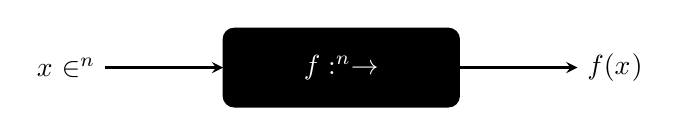
\begin{tikzpicture}
            \draw[rounded corners,fill] (0,0) rectangle (3,1);
            \node[text=white] at (1.5,0.5) {$\obj : \R^n \to \R$};
            \draw[-stealth,thick] (-1.5,0.5) -- (0,0.5);
            \node[left] at (-1.5,0.5) {$\iter \in \R^n$};
            \draw[-stealth,thick] (3,0.5) -- (4.5,0.5);
            \node[right] at (4.5,0.5) {$\obj(\iter)$};
        \end{tikzpicture}
    \end{center}

    \medskip
    
    \begin{block}{}
        \begin{enumerate}
            \item $f$ may be smooth, but derivatives \alert{cannot} be evaluated.
            \item Each function evaluation is \alert{expensive}.
            \item The measure of complexity is the number of \alert{function evaluations}.
            \item Do \alert{not} use DFO if any kind of first order information is available.
        \end{enumerate}
    \end{block}
\end{frame}

\begin{frame}
    \frametitle{Examples of DFO problems}

    \begin{enumerate}
        \item Automatic error analysis \parencite{Higham_1993,Higham_2002}
        \item Tuning nonlinear optimization methods \parencite{Audet_Orban_2006}
        \item \alert<2>{Hyperparameter tuning} \parencite{Ghanbari_Scheinberg_2017}
        \item Censored regression \parencite{Chen_Etal_2018}
        \item Aeroacoustic shape design \parencite{Marsden_2004,Marsden_Etal_2004}
        \item Computational fluid dynamics \parencite{Duvigneau_Visonneau_2004}
        \item \alert<2>{Aircraft engine engineering}~\parencite{Gazaix_Etal_2019}
        \item Rapid-cycling synchrotron accelerator modeling \parencite{Eldred_Etal_2022}
        \item \dots
    \end{enumerate}

    \medskip

    \pause
    \begin{block}{}
        In what follows, we detail two examples from \alert{machine learning} and \alert{MDO}.
    \end{block}
\end{frame}

\begin{frame}
    \frametitle{Hyperparameter tuning in machine learning}

    \begin{center}
        \begin{tikzpicture}
			\uncover<2>{
				\draw[rounded corners,pattern=north east lines,pattern color=DarkOrchid,fill opacity=0.3] (8,3) rectangle (11,4.5);
			}
			\draw[thick,rounded corners] (0,0) rectangle (3,1.5);
			\draw[thick,rounded corners] (0,4) rectangle (3,5.5);
			\draw[thick,rounded corners] (4,2) rectangle (7,3.5);
			\draw[thick,rounded corners] (8,1) rectangle (11,2.5);
			\draw[thick,rounded corners] (8,3) rectangle (11,4.5);
			\draw[thick,-stealth] (3,1) -- (5.5,1) -- (5.5,2);
			\draw[thick] (3,0.5) -- (7.5,0.5) -- (7.5,2.5) -- (7,2.5);
			\draw[thick,-stealth] (7.5,1.75) -- (8,1.75);
			\draw[thick] (3,4.75) -- (7.5,4.75) -- (7.5,3) -- (7,3);
			\draw[thick,-stealth] (7.5,3.75) -- (8,3.75);
			\node at (0.6,0.75) {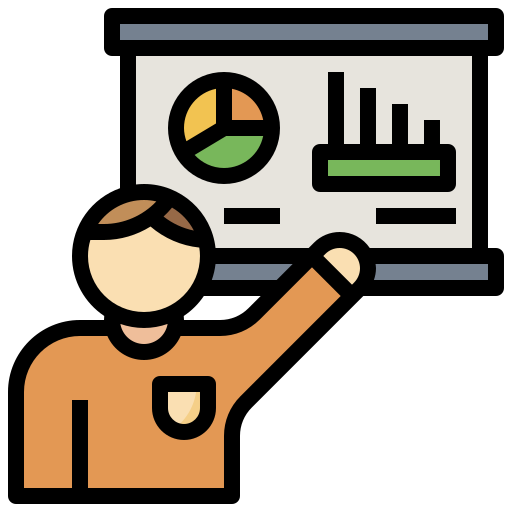
\includegraphics[height=0.75cm]{images/ml/presentation.png}};
			\node at (0.6,4.75) {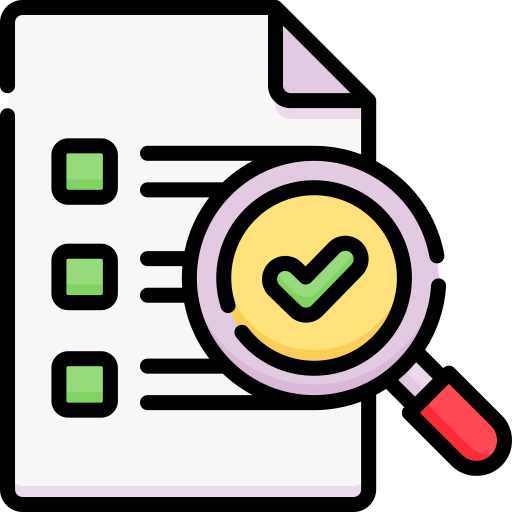
\includegraphics[height=0.75cm]{images/ml/search.png}};
			\node at (4.6,2.75) {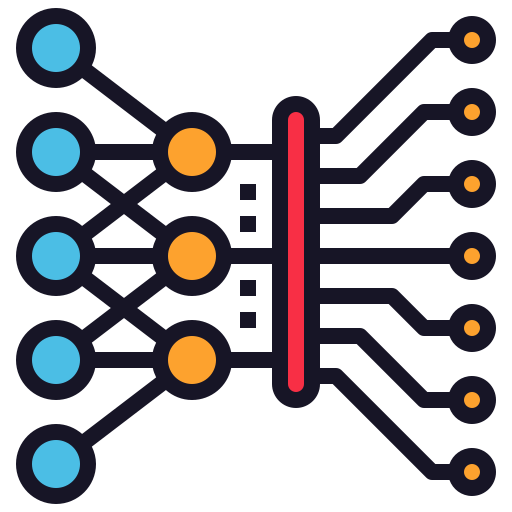
\includegraphics[height=0.75cm]{images/ml/deep-learning.png}};
			\node at (8.6,1.75) {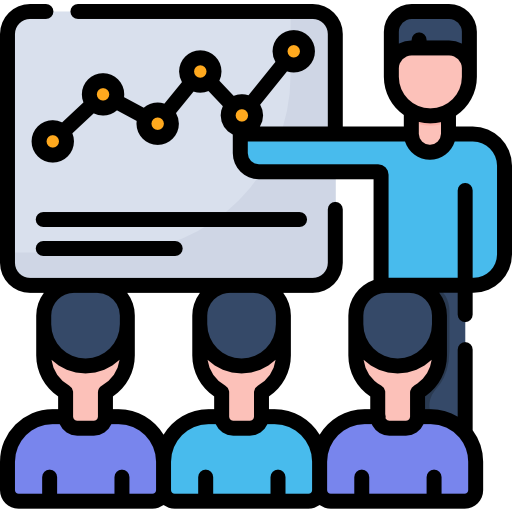
\includegraphics[height=0.75cm]{images/ml/analysis.png}};
			\node at (8.6,3.75) {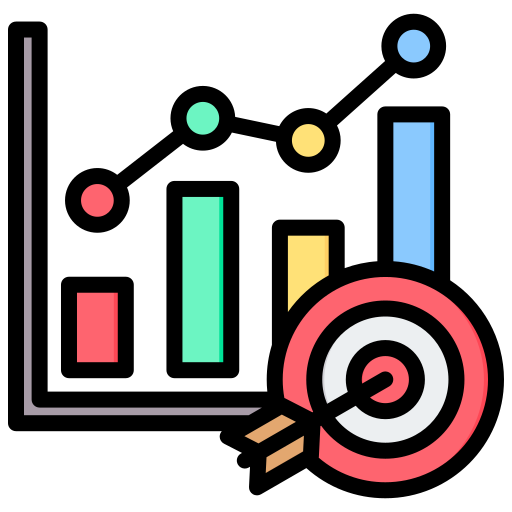
\includegraphics[height=0.75cm]{images/ml/analytics.png}};
			\node at (2,0.75) {\makecell{Training\\ dataset}};
			\node at (2,4.75) {\makecell{Testing\\ dataset}};
			\node at (6,2.75) {\makecell{Machine\\ learning}};
			\node at (10,1.75) {\makecell{Training\\ accuracy}};
			\node at (10,3.75) {\makecell{Testing\\ accuracy}};
			\uncover<2>{
				\draw[rounded corners,pattern=north east lines,pattern color=DarkOrchid,fill opacity=0.3] (0,2) rectangle (3,3.5);
				\draw[thick,rounded corners] (0,2) rectangle (3,3.5);
				\draw[thick,-stealth] (3,2.75) -- (4,2.75);
				\node at (0.6,2.75) {
\includegraphics[height=0.7cm]{images/ml/admin-panel.png}};
				\node at (2,2.75) {\makecell{Hyper-\\ parameters}};
			}
		\end{tikzpicture}
    \end{center}

    \pause
    \begin{block}{}
        \begin{enumerate}
            \item How to \alert{maximize} the testing accuracy by tuning the \alert{hyperparameters}?
            \item What is the \alert{gradient} of the testing accuracy?
        \end{enumerate}
    \end{block}
\end{frame}

\begin{frame}
    \frametitle{Aircraft engine pylon optimization}

    Where to position the engines to maximize the performance of an aircraft?

    \medskip
    
    \begin{center}
        \begin{tikzpicture}
            \draw[thick,rounded corners,pattern=north east lines,pattern color=DarkOrchid,fill opacity=0.3] (0,0) rectangle (3,1.5);
            \draw[thick,rounded corners] (-4,-2.5) rectangle (-1,-1);
            \draw[thick,rounded corners] (0,-2.5) rectangle (3,-1);
            \draw[thick,rounded corners] (4,-2.5) rectangle (7,-1);
            \draw[thick,dotted,rounded corners,DarkOrchid] (-4.25,-2.75) rectangle (7.25,-0.75);
			\draw[thick,stealth-stealth] (1.5,0) -- (1.5,-1);
			\draw[thick,stealth-stealth] (-2.5,-1) -- (-2.5,-0.5) -- (1,-0.5) -- (1,0);
			\draw[thick,stealth-stealth] (5.5,-1) -- (5.5,-0.5) -- (2,-0.5) -- (2,0);
            \node at (1.5,0.75) {\makecell{Multi-disciplinary\\ optimization}};
            \node at (-2.5,-1.75) {\makecell{Aerodynamic\\ optimization}};
            \node at (1.5,-1.75) {\makecell{OAD\\ optimization}};  % Overall Aircraft Design
            \node at (5.5,-1.75) {\makecell{Structure\\ optimization}};
            \node[below right,text=DarkOrchid] at (-4.25,-2.75) {\small\emph{Different independent disciplines/departments}};
        \end{tikzpicture}
    \end{center}
    
	\begin{block}{}
        \begin{enumerate}
            \item Each discipline provides only a \alert{fragment} of the problem.
            \item The derivatives of some or all components involved may be \alert{unknown}.
        \end{enumerate}
    \end{block}
\end{frame}

\begin{frame}
    \frametitle{A lack of theories and methodologies}

    We are in lack of
    \begin{enumerate}
        \item easily usable DFO \alert{solvers}, and
        \item \alert{theoretical} understanding of several DFO techniques.
    \end{enumerate}

    \bigskip

    \begin{block}{Organization of this thesis defense}
        In what follows, we will present
        \begin{enumerate}
            \item the \alert{PDFO} software, interfacing existing widely used methods,
            \item an investigation of a \alert{DFO mechanism} introduced by \textcite{Powell_2006},
            \item new developments in the \alert{SQP method} (derivative-based), and
            \item the \alert{COBYQA} method, a new DFO method.
        \end{enumerate}
    \end{block}
\end{frame}

\section{Solving DFO problems using PDFO}

\begin{frame}
    \frametitle{Existing methods for DFO}

    We want to solve
    \begin{equation*}
        \min_{\iter \in \fset \subseteq \R^n} \obj(\iter),
    \end{equation*}
    where derivatives of~$\obj$ (and possibly the constraint functions) are \alert{unknown}.

    \bigskip

    \begin{block}{}
        \begin{enumerate}
            \item \alert{Direct-search methods}: Nelder-Mead \parencite{Nelder_Mead_1965}, GPS \parencite{Booker_Etal_1999}, MADS \parencite{Audet_Dennis_2006}, \dots
            \item \alert{Model-based methods}: Wedge \parencite{Marazzi_Nocedal_2002}, GALAHAD \parencite{Gould_Orban_Toint_2003}, MNH \parencite{Wild_2008}, \textcite{Fasano_Morales_Nocedal_2009}, \textcite{Jarre_Lieder_2017}, \textcite{Conejo_Karas_Pedroso_2015}, \emph{Powell's methods}, \dots
            % UOBYQA \parencite{Powell_2002}, NEWUOA \parencite{Powell_2006}, BOBYQA \parencite{Powell_2009}, LINCOA \parencite{Powell_2015}, COBYLA \parencite{Powell_1994}, \dots
        \end{enumerate}
    \end{block}
    
	% \begin{enumerate}
    %     \item \textcite{Jarre_Lieder_2017}.
    %     \item \textcite{Santo_Denysiuk_Fernandes_2014}.
    %     \item \textcite{Audet_Digabel_Peyrega_2016}.
    %     \item \textcite{Conejo_Karas_Pedroso_2015}.
    %     \item \textcite{Gould_Orban_Toint_2003}.
    % \end{enumerate}
\end{frame}

\begin{frame}
    \frametitle{A focus on Powell's DFO solvers}
    
	Powell's designed five DFO solvers.

    \medskip

    \begin{center}
        \begin{tabular}{lll}
            \toprule
            Solver  & Feasible set~$\Omega$                                 & References\\
            \midrule
            UOBYQA  & $\R^n$                                                & \textcite{Powell_2002}\\
            NEWUOA  & $\R^n$                                                & \textcite{Powell_2006}\\
            BOBYQA  & $\set{x \in \R^n : \xl \le x \le \xu}$                & \textcite{Powell_2009}\\
            LINCOA  & $\set{x \in \R^n : A x \le b}$                        & \textcite{Powell_2015}\\
            COBYLA  & $\set{x \in \R^n : \con{i}(x) \ge 0, ~ i \in \iub}$   & \textcite{Powell_1994}\\
            \bottomrule
        \end{tabular}
    \end{center}

    \medskip

    \begin{block}{An obstacle to using Powell’s DFO solvers}
        Powell implemented them in \alert{Fortran 77}\dots
    \end{block}
\end{frame}

\begin{frame}
    \frametitle{The need for PDFO}

    \begin{block}{}
        \alert{PDFO} is a \alert{cross-platform} package interfacing Powell's DFO solvers.
    \end{block}

    \medskip

    \begin{enumerate}
        \item The \alert{MATLAB} signature is consistent with \texttt{fmincon}.
        \item The \alert{Python} signature is consistent with \texttt{scipy.optimize.minimize}.
        \item PDFO is \alert{open-source} and distributed under the LGPLv3+ license.
        \item This is \alert{not} a reimplementation of Powell's solvers.
    \end{enumerate}

    \medskip
    
	\begin{center}
        \href{https://www.pdfo.net/}{
\includegraphics[width=0.8in]{images/qr/pdfo.png}}

        \scriptsize\url{https://www.pdfo.net/}
    \end{center}
\end{frame}

\begin{frame}
    \frametitle{Numerical experiments using PDFO}
    
	\begin{columns}
        \begin{column}{0.45\textwidth}
            We compare the solvers
            \begin{enumerate}
                \item on \alert{unconstrained} problems,
                \item from the \alert{CUTEst} set,
                \item of dimension \alert{at most 50}\only<1>{.}\only<2>{,}
                \uncover<2>{
                    \item replacing~$\obj$ with
                    \begin{equation*}
                        \tilde{\obj}(\iter) = [1 + \epsilon(\iter)] \obj(\iter),
                    \end{equation*}
                    with~$\epsilon(x) \sim N(0, \sigma^2)$,~$\sigma = 10^{-2}$.
                }
            \end{enumerate}
        \end{column}
        \begin{column}{0.55\textwidth}
            \begin{center}
                \only<1>{\drawperformanceprofiles{{"NEWUOA","BOBYQA","LINCOA","COBYLA"}}{plain-1-50-perf-newuoa-bobyqa-lincoa-cobyla-u.csv}{4}}%
                \only<2>{\drawperformanceprofiles{{"NEWUOA","BOBYQA","LINCOA","COBYLA"}}{noisy-1-50-2-perf-newuoa-bobyqa-lincoa-cobyla-u.csv}{1}}
            \end{center}
        \end{column}
    \end{columns}
\end{frame}

\section{A lack of DFO theories and methodologies}

\begin{frame}
    \frametitle{Understanding heuristics of DFO methods}
    
	To do.
\end{frame}

\begin{frame}
    \frametitle{The need for new DFO methodologies}
    
	To do.
\end{frame}

\begin{frame}
    \frametitle{The SQP method}
    
	To do.
\end{frame}

\begin{frame}
    \frametitle{A new interpretation of the SQP subproblem}
    
	To do.
\end{frame}

\begin{frame}
    \frametitle{The trust-region SQP method}
    
	To do.
\end{frame}

\begin{frame}
    \frametitle{The \citeauthor{Vardi_1985} approach}

    To define the \alert{trial step}~$\step[k]$,
    \begin{enumerate}
        \item we \alert{shift} the infeasible linear constraints towards~$x^k$, and
        \item we evaluate~$\step[k]$ on the \alert{relaxed subproblem}.
    \end{enumerate}
    
	\begin{columns}
        \begin{column}{0.45\textwidth}
            \begin{center}
                \begin{tikzpicture}
                    % Linear constraints
                    \uncover<1>{\fill[color=RoyalBlue,opacity=0.4] (-4,-1) -- (-1.5,-1) -- (-0.5,4) -- (-4,4) -- cycle;}
                    \uncover<2->{\fill[color=RoyalBlue,opacity=0.4] (-4,-1) -- (-1.175,-1) -- (-0.175,4) -- (-4,4) -- cycle;}
                    \uncover<1>{\fill[color=RoyalBlue,opacity=0.4] (-4,1) -- (0,4) -- (-4,4) -- cycle;}
                    \uncover<2->{\fill[color=RoyalBlue,opacity=0.4] (-4,0) -- (1,3.75) -- (1,4) -- (-4,4) -- cycle;}
        
                    % Trust regions
                    \begin{scope}
                        \clip (-4,-1) rectangle (1,4);
                        \draw[fill=Dandelion,opacity=0.7] (0,0) circle (3);
                    \end{scope}
        
                    % Feasible region for the relaxed subproblem
                    \begin{scope}
                        \clip (-4,0) -- (-15/34,363/136) -- (-0.175,4) -- (-4,4) -- cycle;
                        \uncover<3->{\fill[pattern=north west lines,opacity=0.7] (0,0) circle (3);}
                    \end{scope}
        
                    % Frame and annotations
                    \uncover<4>{
                        \draw[-stealth,thick] (0,0) -- (-0.9,2.7);
                        \node[above right] at (-0.45,1.35) {$\step[k]$};
                    }
                    \draw[fill] (0,0) circle (1.4pt) node[below right] {$\iter[k]$};
                    \draw[thick] (-4,-1) rectangle (1,4);
                \end{tikzpicture}
            \end{center}
        \end{column}
        \begin{column}{0.55\textwidth}
            \begin{tikzpicture}
                \draw[fill=Dandelion,opacity=0.7] (0,0) circle (.2);
                \node[right] at (.4,0) {Trust region};
                \fill[color=RoyalBlue,opacity=0.4] (-.2,-0.8) rectangle (.2,-0.4);
                \node[right] at (.4,-0.6) {Linear constraints};
                \uncover<3->{
                    \fill[pattern=north west lines,opacity=0.7] (-.2,-1.4) rectangle (.2,-1);
                    \node[right] at (.4,-1.2) {Feasible region for~$\step[k]$};
                }
            \end{tikzpicture}
        \end{column}
    \end{columns}
\end{frame}

\begin{frame}
    \frametitle{The \citeauthor{Byrd_1987}-\citeauthor{Omojokun_1989} approach}

    To define the \alert{trial step}~$\step[k]$, we decompose~$\step[k] = \nstep[k] + \tstep[k]$, where
    \begin{enumerate}
        \item the \alert{normal step}~$\nstep[k]$ reduces the (possible) constraint violation, and
        \item the \alert{tangential step}~$\tstep[k]$ reduces the objective function of the subproblem.
    \end{enumerate}
    
    \begin{columns}
        \begin{column}{0.45\textwidth}
            \begin{center}
                \begin{tikzpicture}
                    % Linear constraints
                    \uncover<1-6>{\fill[color=RoyalBlue,opacity=0.4] (-4,-1) -- (-1.5,-1) -- (-0.5,4) -- (-4,4) -- cycle;}
                    \uncover<7>{\fill[color=RoyalBlue,opacity=0.4] (-4,-1) -- (-2.1,-1) -- (-1.1,4) -- (-4,4) -- cycle;}
                    \uncover<1,2>{\fill[color=RoyalBlue,opacity=0.4] (-4,1) -- (0,4) -- (-4,4) -- cycle;}
                    \uncover<3->{\fill[color=RoyalBlue,opacity=0.4] (-4,0.125) -- (1,3.875) -- (1,4) -- (-4,4) -- cycle;}
        
                    % Trust regions
                    \begin{scope}
                        \clip (-4,-1) rectangle (1,4);
                        \draw[fill=Dandelion,draw opacity=0.7,fill opacity=0.5] (0,0) circle (3);
                        \draw[densely dotted,fill=Dandelion,opacity=0.7] (0,0) circle (2.5);
                    \end{scope}
        
                    % Feasible region for the tangential subproblem
                    \begin{scope}
                        \clip (-4,0.125) -- (-27/34,43/17) -- (-0.5,4) -- (-4,4) -- cycle;
                        \uncover<4-6>{\fill[pattern=north west lines,opacity=0.7] (0,0) circle (3);}
                    \end{scope}
                    \begin{scope}
                        \clip (-4,0.125) -- (-1.5,2) -- (-1.1,4) -- (-4,4) -- cycle;
                        \uncover<7>{\fill[pattern=north west lines,opacity=0.7] (0,0) circle (3);}
                    \end{scope}
        
                    % Frame and annotations
                    \uncover<5>{
                        \draw[-stealth,thick,OliveGreen] (-1.5,2) -- (-0.9,2.7);
                        \node[below,xshift=5pt,text=OliveGreen] at (-1.2,2.35) {$\tstep[k]$};
                        \draw[-stealth,thick] (0,0) -- (-0.9,2.7);
                        \node[above right] at (-0.45,1.35) {$\step[k]$};
                    }
                    \uncover<2->{
                        \draw[-stealth,thick,Mahogany] (0,0) -- (-1.5,2);
                        \node[below left,text=Mahogany] at (-0.75,1) {$\nstep[k]$};
                    }
                    \draw[fill] (0,0) circle (1.4pt) node[below right] {$\iter[k]$};
                    \draw[thick] (-4,-1) rectangle (1,4);
                \end{tikzpicture}
            \end{center}
        \end{column}
        \begin{column}{0.55\textwidth}
            \begin{tikzpicture}
                \draw[fill=Dandelion,draw opacity=0.7,fill opacity=0.5] (0,0) circle (.2);
                \node[right] at (.4,0) {Trust region};
                \draw[densely dotted,fill=Dandelion,opacity=0.7] (0,-0.6) circle (.2);
                \node[right] at (.4,-0.6) {Reduced trust region};
                \fill[color=RoyalBlue,opacity=0.4] (-.2,-1.4) rectangle (.2,-1);
                \node[right] at (.4,-1.2) {Linear constraints};
                \uncover<4->{
                    \fill[pattern=north west lines,opacity=0.7] (-.2,-2) rectangle (.2,-1.6);
                    \node[right] at (.4,-1.8) {Feasible region for~$\tstep[k]$};
                }
            \end{tikzpicture}

            \bigskip

            Our \alert<1-6>{new} approach vs. the \alert<7>{standard}\footfullcite{Conn_Gould_Toint_2000} one.
        \end{column}
    \end{columns}
\end{frame}

\begin{frame}
    \frametitle{A connection between the two approaches}
    
	To do.
\end{frame}

\section{Our new DFO method}

\begin{frame}
    \frametitle{The problem addressed by our new DFO method}
    
	To do.
\end{frame}

\begin{frame}
    \frametitle{Inviolable bound constraints}
    
	To do.
\end{frame}

\begin{frame}
    \frametitle{Interpolation-based quadratic models}
    
	To do.
\end{frame}

\begin{frame}
    \frametitle{The derivative-free trust-region SQP method}
    
	To do.
\end{frame}

\begin{frame}
    \frametitle{Our Python implementation}
    
	\begin{center}
        
\includegraphics[width=0.8in]{images/qr/cobyqa.png}
    \end{center}
\end{frame}

\begin{frame}
    \frametitle{Comparison with existing DFO solvers}
    
	To do.
\end{frame}

\section{Conclusion and future research directions}

\begin{frame}
    \frametitle{Conclusion and future research directions}

	To do.
\end{frame}

\appendix

\begin{frame}[t,allowframebreaks]
    \frametitle{References}

	\printbibliography
\end{frame}

\end{document}